\documentclass[12pt, letterpaper]{article}

\usepackage[utf8]{inputenc}  % Basic character encoding
\usepackage{amsmath}         % For mathematical formulas
\usepackage{amssymb}         % Provides an extended symbol collection.
\usepackage{pgfplots}        % For plotting

% personal data
\title{Pre-calculus Notes, MAT 172 Fall 2017}
\author{Eli Heuer}
\date{August 28 - September 03}

% End of preamble
\begin{document}

\maketitle

\section{Introduction}

The well known Pythagorean theorem $x^2 + y^2 = z^2$ was proved to be invalid for other
exponents. Meaning the next equation has no integer solutions:

$$x^n+ y^n = z^n$$

\section{Sets}

In mathematics, a set is a well-defined collection of distinct objects, considered
as an object in its own right. For example, the numbers 2, 4, and 6 are distinct objects
when considered separately, but when they are considered collectively they form a single
set of size three, written {2,4,6}.
\\

\noindent$\mathbb{P}$, denoting the set of all primes: $\mathbb{P}$ = (2, 3, 5, 7, 11, 13, 17, ...)
\\\\
A prime number (or a prime) is a natural number greater than 1 that has no positive
divisors other than 1 and itself. A natural number greater than 1 that is not a prime
number is called a composite number. For example, 5 is prime because 1 and 5 are its
only positive integer factors, whereas 6 is composite because it has the divisors 2 and 3
in addition to 1 and 6.
\\

\noindent$\mathbb{N}$, denoting the set of all natural numbers: $\mathbb{N}$ =
(0, 1, 2, 3, ...)
\\\\
In mathematics, the natural numbers are those used for counting (as in "there are six coins
on the table") and ordering (as in "this is the third largest city in the country").
In common language, words used for counting are "cardinal numbers" and words used for
ordering are "ordinal numbers".
\\

\noindent$\mathbb{Z}$, denoting the set of all integers: $\mathbb{Z}$ =
(..., -2, -1, 0, 1, 2, ...)
\\\\
An integer is a number that can be written without a fractional component.
For example, 21, 4, 0 and -2048 are integers, while 9.75, 5$\frac{1}{2}$ and $\sqrt{2}$ are not.
\\

\noindent$\mathbb{Q}$, denoting the set of all rational numbers: $\mathbb{Q}$ =
(a/b : a, b $\in$ Z, b $\neq$ 0)
\\\\
In mathematics, a rational number is any number that can be expressed as the quotient or fraction p/q of two integers, a numerator p and a non-zero denominator q.
\\

\noindent$\mathbb{R}$, denoting the set of all real numbers.
\\\\
In mathematics, a real number is a value that represents a quantity along a line. The adjective real in this context was introduced in the 17th century by René Descartes, who distinguished between real and imaginary roots of polynomials.
\\

\section{1.1 Rectangular Coordinates}

Just as you can represent real numbers by points on a real number line, you can
represent ordered pairs of real numbers by points in a plane called the
rectangular coordinate system, or the Cartesian plane, named after the French
mathematician René Descartes (1596–1650).
\\
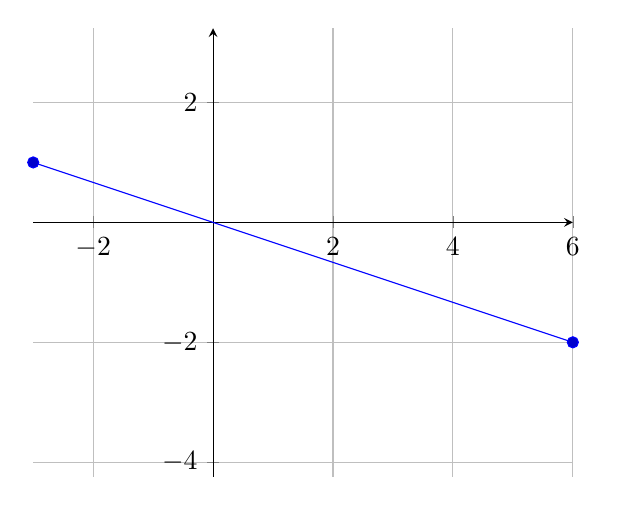
\begin{tikzpicture}
\begin{axis}[axis lines=middle,axis equal,grid=both]
\addplot coordinates{(-3,1) (6,-2)};
\end{axis}
\end{tikzpicture}

\section{Factoring}

The GCF (greatest common factor) of two or more monomials is the product of all their
common prime factors. For example, the GCF of $6x$ and $4x^2$ is $2x$.

\section{Linear Equations}

\end{document}
